Les phases de spécification et d'analyse étant désormais terminées, nous sommes maintenant en mesure de passer à la phase d'implémentation du pipeline OpenHart sur la plateforme DAE.

\section{Implémentation du pipeline}

\subsection{Algorithmes de transcription et de traduction}
Le pipeline OpenHart offre le choix entre trois sortes de tests:
\begin{itemize}
    \item DIR: Teste le programme de transcription uniquement.
    \item DIT: Teste le programme de traduction uniquement.
    \item DTT: Teste les programmes de transcription puis de traduction à la chaîne.
\end{itemize}

La suite de notre travail consiste donc à l'implémentation de deux web-services chaînables offrant la possibilité à l'utilisateur de tester soit son programme de transcription, soit son programme de traduction, soit l'un à la suite de l'autre. 

Par manque de programmes de transcription et de traduction à notre disposition, nous devrons probablement écrire de petits programmes simulant la traduction et la transcription de documents. 


\subsection{Métriques}
Le pipeline OpenHart utilise un ensemble de métriques qui seront implantés à leur tour sur DAE sous forme de web-services. Certains n'évaluent que la transcription, d'autres la traduction. Les webservices chargés d'évaluer la transcription peuvent donc être lancés en parallèle des webservices chargés de lancer la traduction de cette transcription.

\subsection{Pipeline}
Le produit final doit être une chaînage des programmes de transcription/traduction et des métriques testant ces programmes. Dans un premier temps nous avons songé à implémenter un pipeline englobant l'ensemble des phases de l'évaluation, cependant, nous nous sommes redirigés vers un ensemble de plus petits pipelines pour chaque phase dans le but que le produit final soit plus modulaire.

\begin{center}
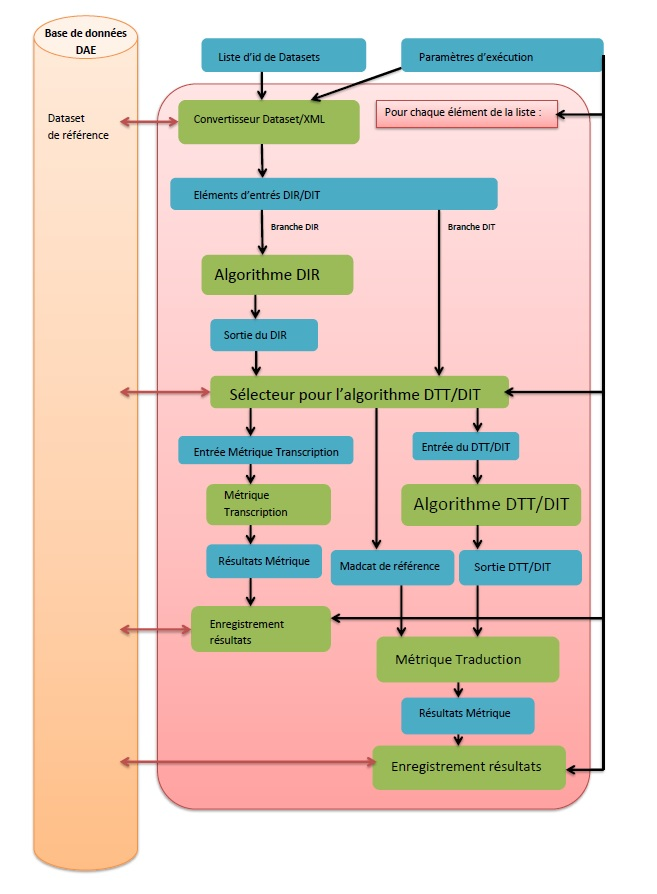
\includegraphics{pipeline}
Première idée de pipeline
\end{center}

\section{Tests à réaliser}

Après la phase d'implémentation du pipeline vient une phase de test et d'étude des éventuelles évolution du produit. Il s'agira dans un premier temps de rechercher d'éventuelles erreurs dans notre travail puis dans un second temps de proposer des améliorations pouvant être apportées au livrable.

\subsection{Recherche d'éventuelles erreurs}
Cette étape du projet consiste à réaliser un ensemble de tests sur le pipeline implémenté afin de détecter d'éventuelles erreurs dans le produit. Un maximum de cas de figures seront étudiés afin d'avoir un pipeline le plus fiable possible. Pour ce faire, nous allons tout d'abord établir un ensemble de scénarios classiques d'utilisation (qui seront par la suite intégrés à la documentation du produit) que nous testerons. Le bon fonctionnement de ces cas est primordial pour que la preuve de
concept à réaliser soit intéressante.   

\subsection{Suggestions d'amélioration}
Il s'agit de l'étape finale de ce projet. Le produit étant une preuve de concept et non une plateforme définitive, nous devrons réfléchir aux possibilités d'amélioration et d'évolution de cette plateforme. Le résultat de cette étape se traduira par un document relatant s'ensemble de nos suggestions d'améliorations qui sera fourni à notre client. Ceci sera utile pour les prochaines personnes qui travailleront sur ce projet. De plus, le produit final étant présenté comme une preuve de concept au NIST, il est également intéressant de leur présenter l'ensemble des améliorations et évolutions que peut connaître cette plateforme.
N
